%----------------------------------------------------------------------------
\chapter{Rendszerterv}\label{sect:rszterv}
%----------------------------------------------------------------------------

Jelen fejezetben szeretnénk bemutatni az elkészítendő rendszer tervét. Az egyes szakaszok kitérnek az architektúra kiválasztására és megvalósítására (\sectref{architektura} szakasz), az itt szereplő rétegek tervezésére és bemutatására (\sectref{retegek} szakasz), valamint végül a program funkcióinak ismertetésére (\sectref{rsz_funkciok} szakasz).

%,,,,,,,,,,,,,,,,,,,,,,,,,,,,,,,,,,,,,,,,,,,,,,,,,,,,,,,,,,,,,,,,,,,,,,,,,,,,
\section{Architektúra}\label{sect:architektura}
%,,,,,,,,,,,,,,,,,,,,,,,,,,,,,,,,,,,,,,,,,,,,,,,,,,,,,,,,,,,,,,,,,,,,,,,,,,,,

A program architektúrájának a \sectref{tervarch} szakaszban említett háromrétegű (multitier) architektúrát választottuk. Ezzel a megoldással a felhasználói felület adminisztrálásának terhét le tudjuk venni a kiszolgáló válláról, az csak az alkalmazás hosztolásában, illetve az esetleges működés közbeni kommunikációban vesz részt.

%. . . . . . . . . . . . . . . . . . . . . . . . . . . . . . . . . . . . . .
%\subsubsection{Egy subsubsection}\label{sect:egysubsubsection}
%. . . . . . . . . . . . . . . . . . . . . . . . . . . . . . . . . . . . . .

%,,,,,,,,,,,,,,,,,,,,,,,,,,,,,,,,,,,,,,,,,,,,,,,,,,,,,,,,,,,,,,,,,,,,,,,,,,,,
\section{Rétegek}\label{sect:retegek}
%,,,,,,,,,,,,,,,,,,,,,,,,,,,,,,,,,,,,,,,,,,,,,,,,,,,,,,,,,,,,,,,,,,,,,,,,,,,,

Ebben a szakaszban szeretnénk egyesével, röviden bemutatjuk az elkészült program háromrétegű architektúrájának rétegeit, azok felépítését. Az implementáció részleteibe csak a szükséges mélységig merülünk bele, a cél inkább a tervezési szempontok, logikai működés bemutatása.

%............................................................................
\subsection{Kliens réteg}\label{sect:kliens_reteg}
%............................................................................

Az alkalmazás kliens rétegében (vagyis a felhasználó számítógépén) fut az elkészített alkalmazásunk Microsoft Silverlight-ban készített része.

A Silverlight alkalmazások logikailag két részre bonthatók. Egyrészt a felhasználói interfész egyes részeit XAML (eXtensible Application Markup Language) formátumú fájlok írják le, a felület alatt futó alkalmazás pedig (eseménykezelőkkel összekapcsolva a kettőt) változatos CLI nyelveken programozható. A mi választásunk ezek közül a C\#-ra esett.

\bigskip

Az alkalmazás főablakát a \texttt{MainPage.xaml}-ben található \texttt{UserControl} objektum alkotja. Ebbe vannak beágyazva az egyes funkciókat megvalósító további \texttt{UserControl} objektumok, melyek grafikusan általában egy-egy lekerekített szélű narancssárga dobozban valósulnak meg (lásd \figref{alk_felulet} ábra).

\begin{figure}[!ht]
\centering
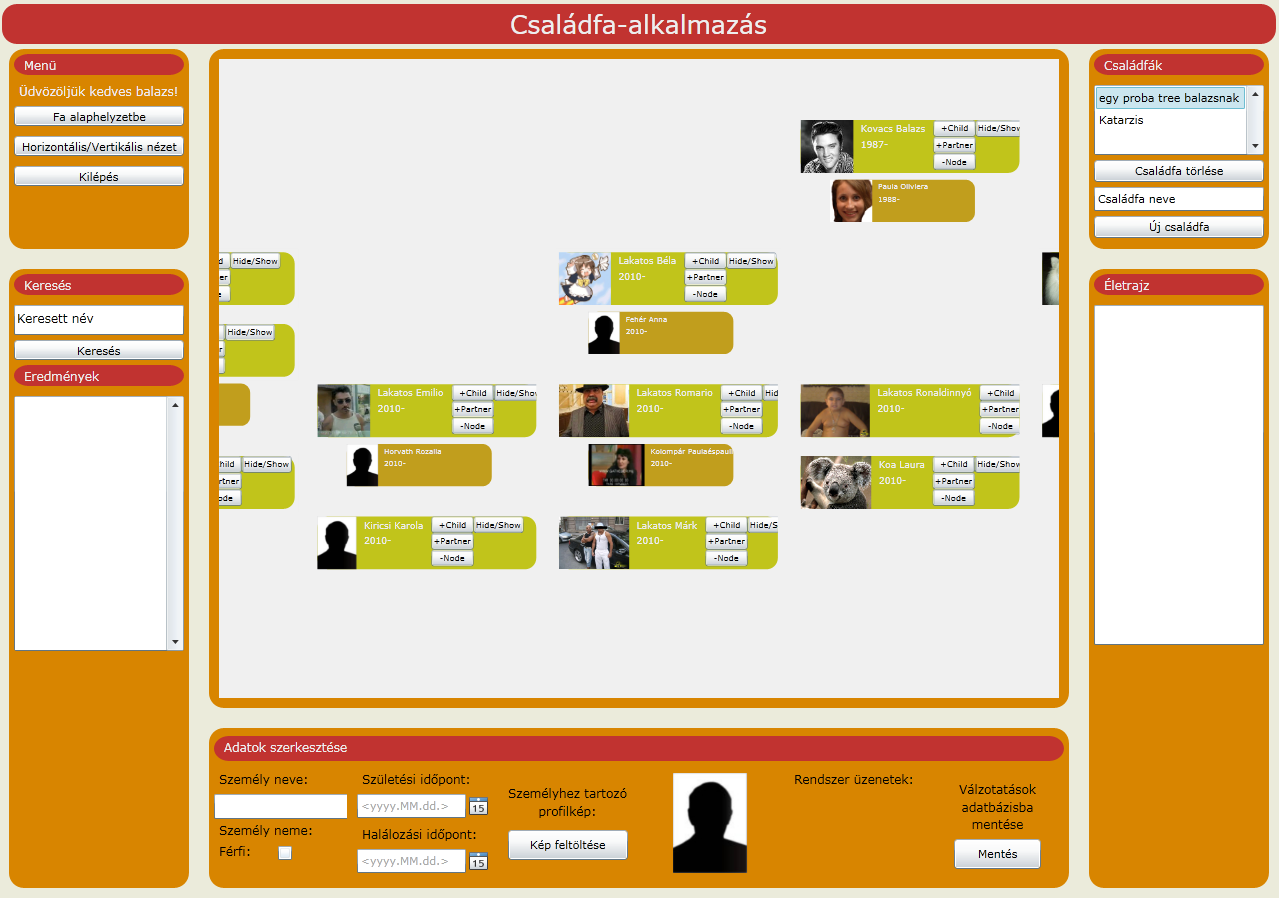
\includegraphics[width=130mm, keepaspectratio]{figures/felulet.png}
\caption{Az alkalmazás főablaka.}
\label{fig:alk_felulet}
\end{figure}

A kezelőfelület elemeinek összefogásán kívül az alkalmazás \texttt{MainPage.xaml.cs} forrásfájljában végezzük a megjelenített családfa mozgatását, illetve nagyítását, kicsinyítését az egérre való húzáshoz, illetve az egérgörgő mozgásához kapcsolt eseménykezelő függvények megvalósításával.

\bigskip

\begin{figure}[!ht]
\centering
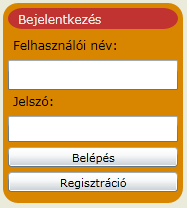
\includegraphics[width=50mm, keepaspectratio]{figures/login.png}
\caption{A bejelentkezésre szolgáló dobozo képe.}
\label{fig:alk_login}
\end{figure}

A \texttt{LoginControl.xaml} és \texttt{LoginControl.xaml.cs} fájlok a bal felső sarokban található menüdoboz doboz kinézetét és működését írják le. Itt történik a felhasználó beléptetése, ha érvényes név és jelszó páros birtokában van, valamint itt, a doboz legalján kapott helyet a regisztrációs ablak megnyitására szolgáló gomb is, ahogy a \figref{alk_login} ábrán is látható.

\bigskip

A \texttt{RegistrationControl} objektum alá rendeltük az új felhasználók regisztrálásához szükséges felugró ablakot, valamint a megfelelően kitöltött regisztrációs űrlap esetén a tényleges regisztrációt. A doboz képét a \figref{alk_register} ábra mutatja.

\begin{figure}[!ht]
\centering
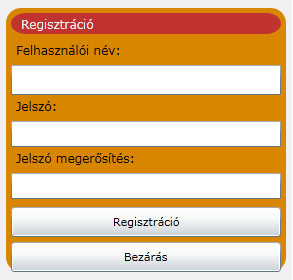
\includegraphics[width=50mm, keepaspectratio]{figures/register.png}
\caption{A regisztrációs ablak.}
\label{fig:alk_register}
\end{figure}

\bigskip

A \texttt{TreeSelector} objektum grafikus megjelenése egy választóablak, amelyben a felhasználó a rendszerben elmentett családfái (ugyanis egy felhasználóhoz több családfa is tartozhat) között navigálhat, újat vehet fel, esetleg törölheti a kiválasztottat. A doboz képe a \figref{csaladfa_panel} ábrán látható.

\begin{figure}[!ht]
\centering
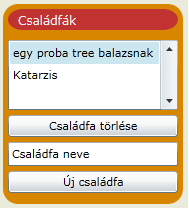
\includegraphics[width=45mm, keepaspectratio]{figures/csaladfa-panel.png}
\caption{A felhasználó családfáinak menedzselésére szolgáló panel.}
\label{fig:csaladfa_panel}
\end{figure}

\bigskip

A középen megjelenített családfa egy \texttt{TreeHandler} objektumba megfelelő módon beágyazott \texttt{TreeNode} csomópontok halmaza. A felhasználó által kiválasztott családfa felépítése a \texttt{TreeHandler.xaml.cs} forrásfájl idetartozó függvényei segítségével történik. Új személyek felvétele a fa megfelelő elemein elhelyezett gombokkal lehetséges. Egy példa családfát mutat a \figref{alk_tree} ábra.

\begin{figure}[!ht]
\centering
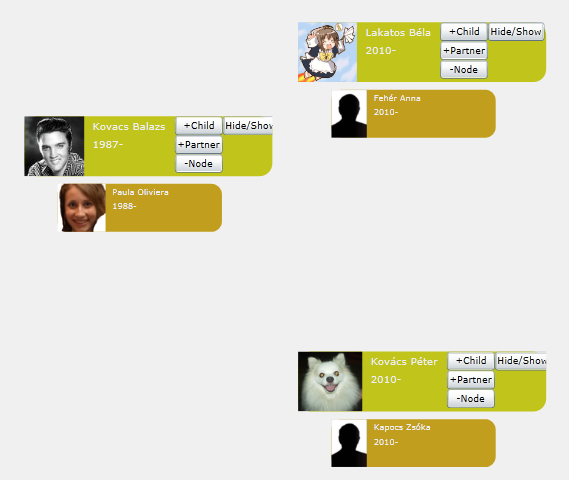
\includegraphics[width=80mm, keepaspectratio]{figures/famtree.png}
\caption{Példa egy, a program által megjelenített családfára.}
\label{fig:alk_tree}
\end{figure}

\bigskip

A \texttt{NodeEditor} objektum által képviselt dobozban van lehetőség a kiválasztott személy adatait módosítani. A módosítható tulajdonságok között van a felhasználó születési és halálozási ideje, valamint a személyt reprezentáló avatár. Az adatbázis, és a felület tervezése során figyelmet fordítottunk arra, hogy a rendszer igény szerint könnyen bővíthető legyen más, a felhasználók által szükségesnek tartott adat tárolásával.

A doboz automatikusan kitöltődik a kiválasztott személy adataival (a kiválasztást az illető képére való kattintással tudjuk előidézni). Az aktív személy szerkeszthető adatait mutatja a \figref{alk_edit} ábra.

\begin{figure}[!ht]
\centering
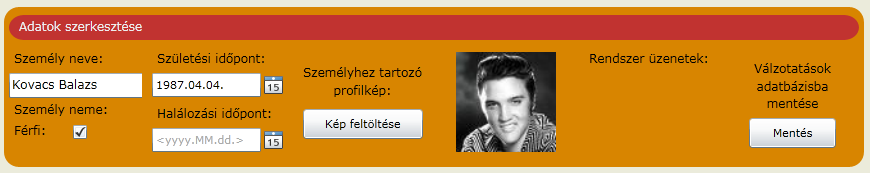
\includegraphics[width=100mm, keepaspectratio]{figures/reszletek.png}
\caption{Egy személy részletes adatai.}
\label{fig:alk_edit}
\end{figure}

%............................................................................
\subsection{Webszerver réteg}\label{sect:szerver_reteg}
%............................................................................

Az alkalmazás szerver rétegét egy Microsoft IIS webszerver szolgálja ki. A Silverlight program a böngészőablak teljes hasznos területét elfoglalja, ezen felül más statikus (HTML) vagy dinamikus (ASP) elemeket az oldal nem tartalmaz. Ennek megfelelően ezen réteg funkciója kizárólag a Silverlight-alkalmazás hosztolására korlátozódik.

%............................................................................
\subsection{Adatbázis réteg}\label{sect:adatbazis_reteg}
%............................................................................

Az adatbázis réteg -- nevéből adódóan -- szolgáltatja az alkalmazás hátterében futó adatbázist, amelyben a felhasználói adatok találhatók. Sémája a \figref{db_sema} ábrán látható.

\begin{figure}[!ht]
\centering
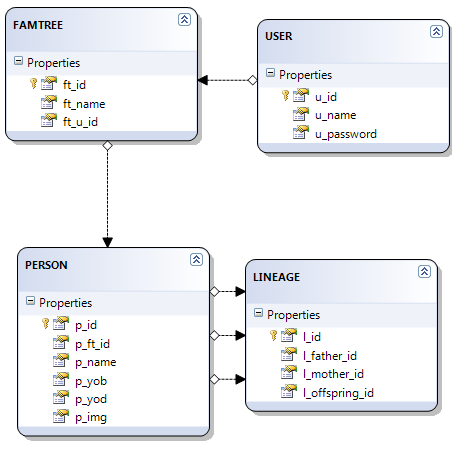
\includegraphics[width=70mm, keepaspectratio]{figures/db_sema.png}
\caption{Az adatbázis réteg felépítése.}
\label{fig:db_sema}
\end{figure}

A \texttt{USERS(\textbf{u\_id}, u\_name, u\_password)} tábla elsődleges kulcsa a \texttt{u\_id} mező, ez egy rendszer által automatikusa generált felhasználói azonosítót tartalmaz. Az \texttt{u\_name} mező a felhasználói nevet tartalmazza, ez szintén egyedi, viszont esetleg megváltoztatható -- ezért különítettük el a felhasználó tevékenysége során végig állandó felhasználói azonosítótól. Az \texttt{u\_password} mező végzetül a felhasználó jelszavának hash-ét tartalmazza.

Mivel egy-egy felhasználó több családfát is létrehozhat, ezért a \texttt{FAMTREE(ft\_id, ft\_name, ft\_u\_id)} táblában eltároljuk, hogy az egyedi azonosítójú (\texttt{ft\_id} -- elsődleges kulcs) családfa melyik felhasználóhoz tartozik, a \texttt{ft\_u\_id} külső kulcs (foreign key) segítségével. Ezen felül minden rekordban eltároljuk a fa elnevezését is, a könnyebb felhasználói azonosíthatóság végett.

A \texttt{PERSON(p\_id, p\_ft\_id, p\_name, p\_yob, p\_yod, p\_img)} tábla rekordjaiban tároljuk a családfákban szereplő személyek adatait. Minden személynek egyedi azonosítója van, ez a tábla \texttt{p\_id} elsődleges kulcsa. Külső kulcsként megjelenik annak a családfának az azonosítója, amelyhez az adott személy tartozik, erre szolgál a \texttt{p\_ft\_id} mező. Ezen kapcsolat segítségével lehet a felvett személyeket a rendszer felhasználóihoz is kötni (a \texttt{FAMTREE} tábla megfelelő külső kulcsán keresztül). A rekordok ezen felül a személyes adatokat tartalmazzák, úgymint a születés és az esetleges elhalálozás éve, név, valamint egy adatbázisban tárolt kép.

Végül a családfákban szereplő személyek közötti kapcsolatot a \texttt{LINEAGE(l\_id, l\_father\_id, l\_mother\_id, l\_offspring\_id)} tábla teremti meg. Ebben minden kapcsolat egy egyedi azonosítóval rendelkezik (ez a lekérdezés \texttt{l\_id} elsődleges kulcsa), és egy szülő-gyerek kapcsolatot ír le három külső kulcs segítségével. Az itt megadott apa--anya--gyermek hármas segítségével minden hagyományos rokoni kapcsolat leírható, majd a táblákat megfelelően illesztve a leszármazások faszerkezete lekérdezhető.

\bigskip

A fentiekben nem tértünk ki külön az egyes mezők típusára, illetve hosszára. Tettük ezt azért, mert az esetek nagy részében azonosítókkal, illetve rövid szöveges mezőkkel dolgoztunk. Ezek típusa egységesen egész szám (\texttt{INT}), illetve 50 karakter hosszúságú karakterlánc (\texttt{VARCHAR(50)}). Egyedüli kivételt a felhasználói képeket tartalmazó \texttt{p\_img} mező jelent ennek típusa a beépített \texttt{IMAGE} típus.

%,,,,,,,,,,,,,,,,,,,,,,,,,,,,,,,,,,,,,,,,,,,,,,,,,,,,,,,,,,,,,,,,,,,,,,,,,,,,
\section{Funkciók}\label{sect:rsz_funkciok}
%,,,,,,,,,,,,,,,,,,,,,,,,,,,,,,,,,,,,,,,,,,,,,,,,,,,,,,,,,,,,,,,,,,,,,,,,,,,,

A program lehetővé teszi, hogy felhasználók regisztráljanak, majd választott felhasználói nevüket és jelszavukat használva beléphessenek a programba. Az alkalmazáson belül lehetőségük van családfákat létrehozni, illetve menedzselni.

A középső panelen az aktuális családfa látható megjelenítve, ez mozgatható illetve nagyítható/kicsinyíthető. A kiválasztott személy életrajzi adatai a jobb oldalon található ,,Életrajz'' dobozban kerülnek megjelenítésre.

Új személy hozzáadására, vagyis a fa építésére a már meglévő csomópontokra támaszkodva van lehetőség. A csomópontokban található gombok megnyomásával lehet új személyt felvenni a fába, a személyhez házastársat rendelni, valamint a kiválasztott személyt (és leszármazottait) törölni a családfából.

A jobb felső, ,,Családfák'' feliratú dobozban van lehetőség a bejelentkezett felhasználó családfái közötti navigálásra, új létrehozására, vagy a kiválasztott családfa törlésére.

A családfákban szereplő személyek közötti keresés valósítható meg a bal oldalon, a menüdoboz alatt elhelyezett ,,Keresés'' feliratú dobozban. A keresés névtöredékre történhet, az eredmények a keresőmező alatti fehér hátterű listadobozban kerülnek megjelenítésre. A listában az egyes eredményekre kattintva, a megfelelő személy kerül kiválasztásra a családfában.
